\documentclass[twocolumn,a4paper,11pt]{scrartcl}

% Language and font encoding
\usepackage[spanish,es-noshorthands]{babel}
\usepackage[utf8]{inputenc}
\usepackage[T1]{fontenc}

% Other necessary packages
\usepackage{graphicx}
\usepackage{amsmath}
\usepackage{cite}

% Additional formatting for two-column layout with centered abstract
\renewcommand{\absnamepos}{empty}  % Remove space where "Abstract" title was
\addto{\captionsspanish}{\renewcommand{\abstractname}{}} % quitar título del resumen

% Title information
\title{Constante de Planck}
\author{Nombre del Autor}
\date{}

\begin{document}

\twocolumn[
  \begin{@twocolumnfalse}
    \maketitle
    \begin{abstract}
        \begin{center}
        \begin{minipage}{0.6\textwidth}
    Este trabajo presenta un estudio en el que determinamos experimentalmente la constante de Planck por medio del efecto fotoeléctrico. Utilizando una lámpara de mercurio y un montaje de detección fotoeléctrica, se midieron las corrientes generadas por electrones emitidos bajo la influencia de diferentes frecuencias de luz. Se aplicó un potencial de frenado permitiendo establecer una relación lineal entre el potencial de frenado y la frecuencia de los fotones incidentes. Los resultados obtenidos proporcionan un valor experimental de la constante de Planck que coincide con el orden valor teórico aceptado.
    \end{minipage}
    \end{center}
    \end{abstract}
\end{@twocolumnfalse}
]

\section{Objetivos}
Nos proponemos examinar cómo diferentes longitudes de onda dentro del espectro visible interactúan con una superficie fotosensible, observando las variaciones en la emisión de electrones. Además, investigaremos el impacto de un potencial de frenado aplicado a una celda fotoeléctrica, analizando cómo este afecta el comportamiento de los electrones emitidos. Finalmente, buscaremos obtener un valor experimental de la constante de Planck.

\section{Marco teórico}

El efecto fotoeléctrico ocurre cuando un fotón interactúa con los electrones de un metal, transfiriendo su energía y potencialmente liberando el electrón del átomo. La energía del fotón, dada por $E = h\nu$, donde $h$ es la constante de Planck y $\nu$ es la frecuencia de la luz, debe ser suficiente para superar la función de trabajo del metal y proporcionar energía cinética al electrón emitido.

La relación entre la energía del electrón emitido ($E_e$), la energía del fotón incidente, y la función de trabajo del metal ($\phi$) se expresa mediante la ecuación:

\begin{equation}
E_e = h\nu - e\phi
\end{equation}

donde $e$ representa la carga del electrón.

Para medir esta energía de los electrones emitidos, se emplea un potencial de frenado ($V_f'$) entre el cátodo (metal emisor) y el ánodo (metal colector). El flujo de electrones entre estos electrodos cesa cuando:

\begin{equation}
E_e = eV_f'
\end{equation}

Este flujo de electrones genera una pequeña corriente ($I_C$).

Es importante considerar que tanto el cátodo como el ánodo poseen funciones de trabajo que afectan el movimiento de los electrones. Por lo tanto, el potencial de frenado efectivo ($V_f'$) se relaciona con el potencial aplicado ($V_f''$) mediante:

\begin{equation}
V_f' = V_f'' + (\phi_A - \phi_C)
\end{equation}

donde $\phi_A$ y $\phi_C$ son las funciones de trabajo del ánodo y cátodo respectivamente.

Combinando las ecuaciones (1), (2) y (3), obtenemos una relación lineal entre el potencial aplicado y la frecuencia de los fotones incidentes:

\begin{equation}
V_f'' = (h/e)\nu - \phi_A
\end{equation}

Esta ecuación nos permite determinar la constante de Planck. Al graficar el potencial aplicado en el que cesa el flujo de electrones ($I_C = 0$) contra la frecuencia de los fotones incidentes, obtendremos una línea recta cuya pendiente es $h/e$ y cuya intersección con el eje vertical nos da la función de trabajo del ánodo.

\section{Diseño experimental}

El montaje experimental para medir la constante de Planck se muestra en la Figura \ref{fig:montaje}.

\begin{figure}[h]
    \centering
    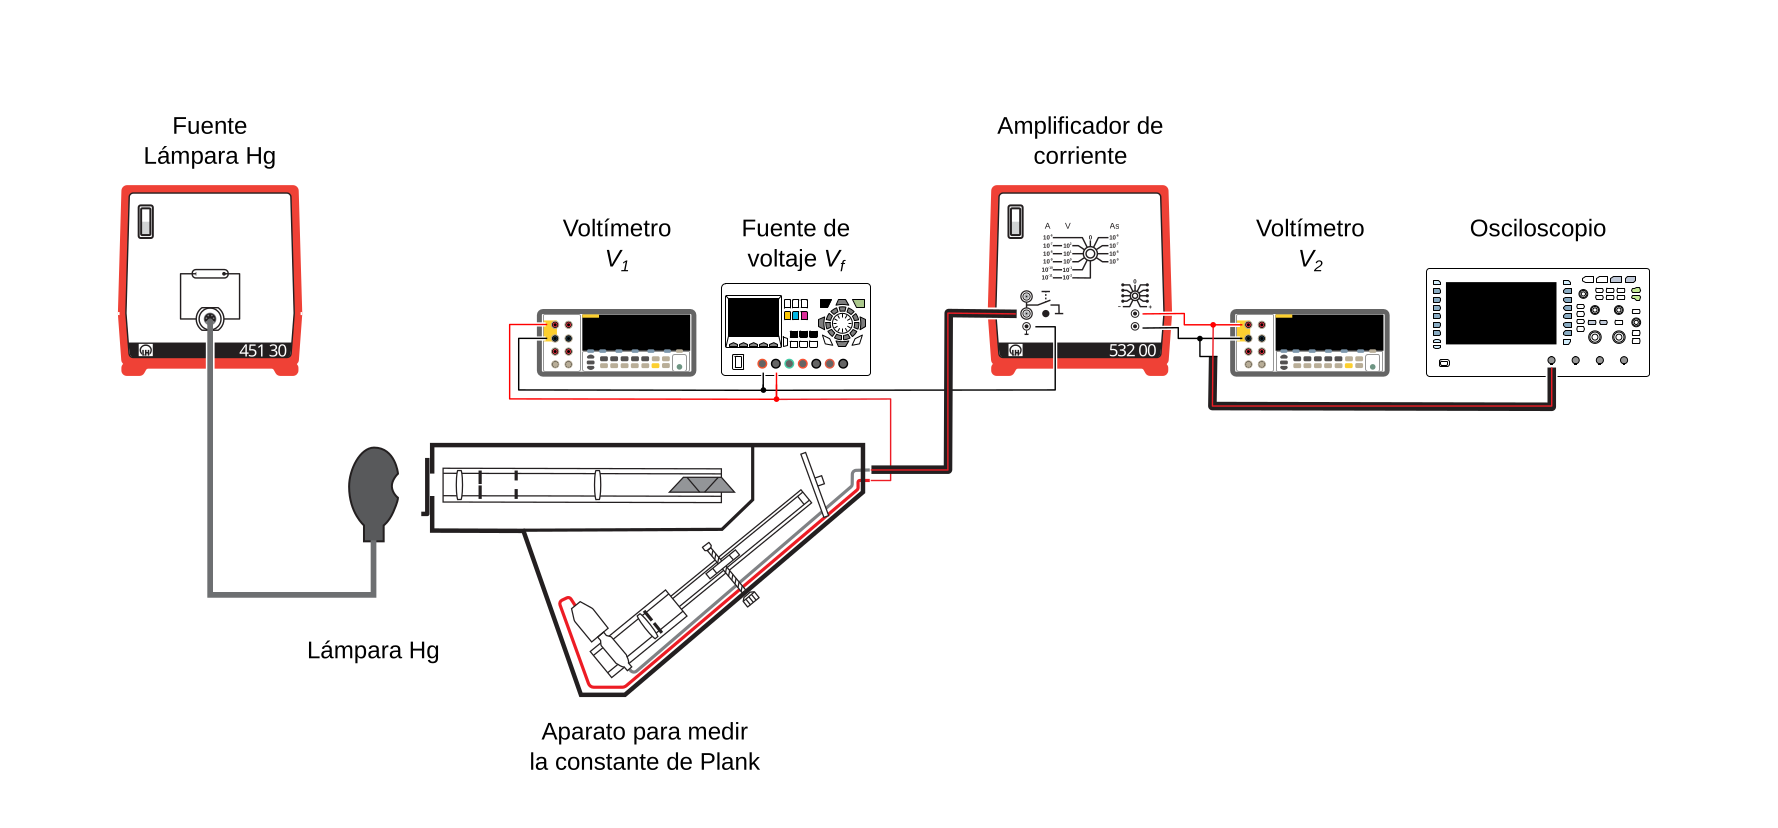
\includegraphics[width=0.8\linewidth]{montaje_experimental_const_planck.png}
    \caption{Esquema del montaje experimental para medir la constante de Planck}
    \label{fig:montaje}
\end{figure}

Una lámpara de mercurio sirve como fuente de fotones. La luz emitida por esta lámpara se hace pasar a través de un prisma, que separa el haz en líneas de emisión discretas con frecuencias conocidas. Estas líneas de diferentes colores corresponden a las distintas transiciones electrónicas en los átomos de mercurio.

Cada una de estas líneas espectrales se dirige, de manera individual y secuencial, hacia el cátodo de una fotocelda. Este proceso permite estudiar el efecto fotoeléctrico para diferentes frecuencias de luz incidente. La fotocelda está conectada a un circuito que incluye un amplificador y una fuente de voltaje variable.

El amplificador permite la detección de la pequeña corriente $I_c$ generada por el flujo de electrones desde el cátodo al ánodo de la fotocelda. Esta corriente, producto directo del efecto fotoeléctrico, se amplifica y se convierte en una señal de voltaje proporcional, facilitando su medición precisa.

La fuente de voltaje variable se utiliza para aplicar un potencial de frenado $V_f$ entre el cátodo y el ánodo de la fotocelda. Este potencial de frenado permite determinar la energía cinética máxima de los electrones emitidos.

El procedimiento a seguir es:

\begin{enumerate}
    \item Montar el experimento como se muestra en la figura 1.
    \item Encender la lámpara de mercurio por medio de la fuente de esta. Esperar al menos 5 minutos a que esta caliente y alcance su máximo de emisión.
    \item Retirar la tapa de entrada de luz del aparato para medir la constante de Planck.
    \item Retirar el prisma de visión directa del aparato para medir la constante de Planck y enfocar una línea bien definida en el colimador que se encuentra en la lente justo antes de la fotocelda. Puede utilizar una hoja de papel sobre el colimador para lograr esto.
    \item Colocar nuevamente el prisma de visión directa y verificar que todas las líneas de emisión puedan alcanzar la fotocelda por medio de rotar el espejo colocado en el aparato para medir la constante de Planck.
    \item Hacer incidir una de las líneas de la lámpara de mercurio en la fotocelda. Tomar nota del color que se hace incidir.
    \item Tapar la entrada de luz de la lámpara de mercurio y cerrar completamente el aparato para medir la constante de Planck.
    \item Encender el osciloscopio:
    \begin{enumerate}
        \item Configurar el osciloscopio para un barrido temporal lento, en el rango de 100 ms a 500 ms por división.
        \item Ajustar la escala vertical de voltaje en el rango de unos mV por división.
    \end{enumerate}
    \item Encender el multímetro V2.
    \item Encender el amplificador y colocar el selector en el máximo valor de amplificación para corriente. Tomar nota de este valor.
    \item Medir por medio del multímetro V2 y el osciloscopio el voltaje de salida del amplificador. Ajustar por medio de la perilla de offset de la salida del amplificador, un valor lo más cercano a cero posible.
    \item Configurar en el multímetro V2 la función de análisis estadístico de este para tomar 200 muestras.
    \item Realizar por medio del multímetro V2 la medición del valor de corriente cero.
    \item Encender la fuente de voltaje Vf y el multímetro V1.
    \item Configurar la salida de la fuente de voltaje para cero voltios.
    \item Configurar en el multímetro V1 la función de análisis estadístico de este para tomar 100 muestras.
    \item Destapar la entrada de luz de la lámpara de mercurio del aparato para medir la constante de Planck.
    \item Realizar mediciones del valor de corriente IC vs Vf para valores de Vf de 0 a -1.5 V en intervalos de 0.1 V, por medio del siguiente procedimiento:
    \begin{enumerate}
        \item Configurar el valor deseado de potencial de frenado en la fuente de voltaje.
        \item Observar en el osciloscopio el comportamiento del voltaje de salida del amplificador. Cuando este sea estable se procede con las siguientes mediciones.
        \item Medir el valor de la corriente IC por medio del multímetro V2. Anotar el valor medio y la desviación.
        \item Medir el valor del potencial de frenado por medio del voltímetro V1. Anotar el valor medio y la desviación.
    \end{enumerate}
    \item Repetir a partir del paso 6 para otro color, hasta tener las curvas IC vs Vf para al menos 4 colores diferentes.
\end{enumerate}


\section{Resultados y discusión}

\subsection{Curvas de $I_C$ vs $V_f$ para diferentes colores}

La Figura \ref{fig:ic_vs_vf} muestra las curvas de corriente $I_C$ en función del potencial de frenado $V_f$ para cinco colores diferentes de luz incidente. Cada curva representa una longitud de onda específica de la lámpara de mercurio utilizada en el experimento.

\begin{figure}[h]
    \centering
    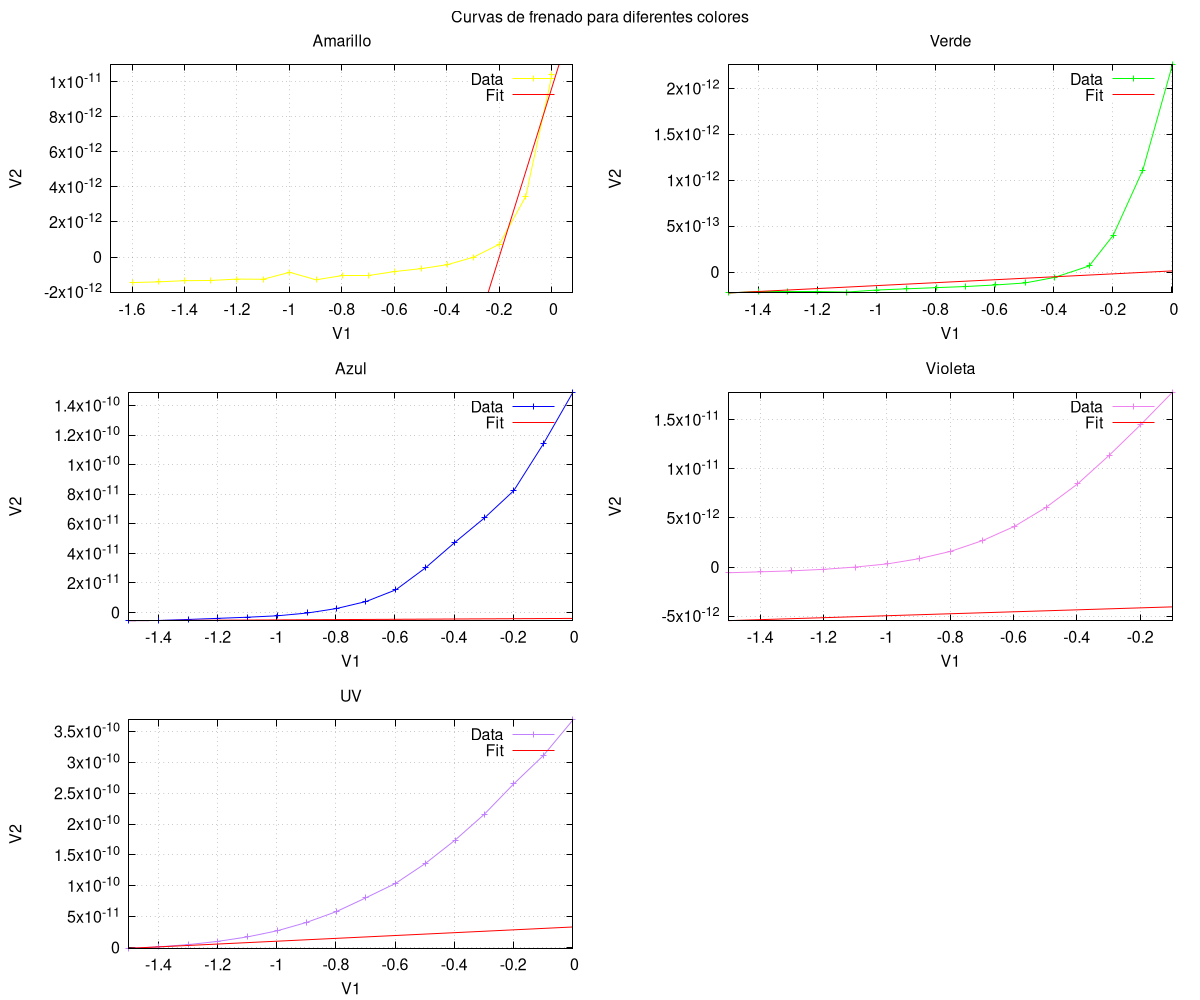
\includegraphics[width=0.8\linewidth]{planck_constant_fits.png}
    \caption{Curvas de $I_C$ vs $V_f$ para diferentes colores de luz, a escala de E-12.}
    \label{fig:ic_vs_vf}
\end{figure}

Estas curvas permiten observar cómo el potencial de frenado afecta la corriente de electrones emitidos.

Para determinar el potencial de frenado de cada color de luz utilizamos el método descrito por Melissinos \cite{melissinos1966} según el cual tomamos el ajuste lineal de cada una de las ramas y tomamos el potencial correspondiente a la intersección de los dos ajustes como el voltaje de frenado para cada color.

\subsection{Datos de $V_f$ y frecuencia}

La Tabla \ref{tab:vf_frecuencia} presenta los valores de potencial de frenado $V_f$ y las frecuencias correspondientes de los fotones incidentes para cada color de luz utilizado en el experimento.

\begin{table}[h]
\centering
\caption{Valores de $V_f$ y frecuencia para diferentes colores de luz.}
\label{tab:vf_frecuencia}
\begin{tabular}{|c|c|c|}
\hline
Color & Frecuencia (THz) & $|V_f|$ (V) \\
\hline
Amarillo & 519 & 0.1570 \\
Verde & 549 & 0.2833 \\
Azul & 688 & 0.5903 \\
Violeta & 741 & 0.7058 \\
UV & 822 & 0.8949 \\
\hline
\end{tabular}
\end{table}

\subsection{Ajuste de $V_f$ vs frecuencia}

La Figura \ref{fig:vf_vs_frecuencia} muestra el ajuste lineal entre el potencial de frenado $V_f$ y la frecuencia de los fotones incidentes.

\begin{figure}[h]
    \centering
    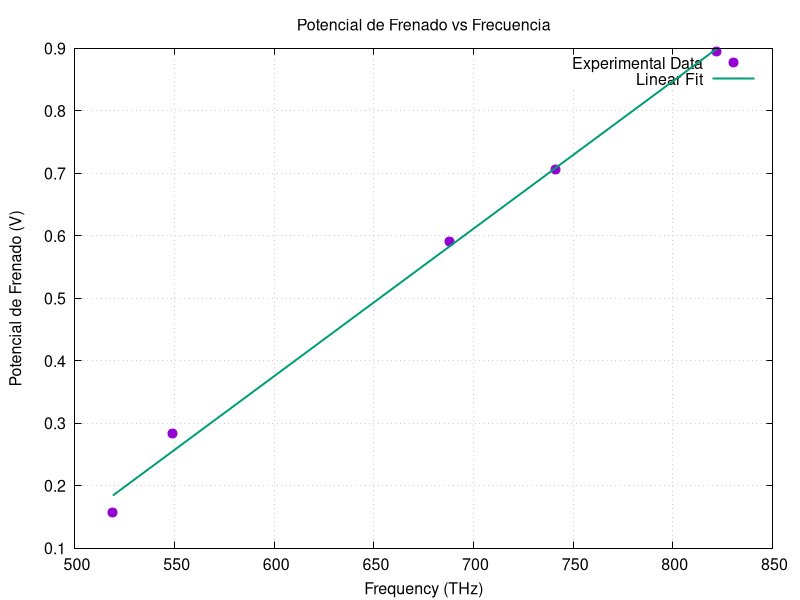
\includegraphics[width=0.8\linewidth]{vf_vs_frecuencia.png}
    \caption{Ajuste lineal de $V_f$ vs frecuencia.}
    \label{fig:vf_vs_frecuencia}
\end{figure}

\subsection{Determinación de la constante de Planck}

Para determinar la constante de Planck, utilizamos la ecuación lineal obtenida del ajuste de $V_f$ vs frecuencia:

\begin{equation}
V_f = \left(\frac{h}{e}\right) \nu - \phi_A
\end{equation}

La pendiente de la línea ajustada nos proporciona el valor de $\frac{h}{e}$. Multiplicando esta pendiente por la carga del electrón $e$, obtenemos el valor experimental de la constante de Planck $h = (3.24 \pm 0.34)E-34$. Lo cual debemos contrastar con el valor teórico aceptado de $h = 6.6E-34$ y verificar que con este método sólamente hemos sido capaces de verificar el orden de la constante, pero no su valor exacto.

\section{Conclusiones}

Nuestro experimento no nos ha permitido determinar el valor de la constante de Planck con precisión más allá del orden de la misma.

Este resultado subraya cuan sensible es nuestro montaje experimental a la hora de obtener las mediciones necesarias para encontrar la constante de Planck.

Además, el experimento ha proporcionado una oportunidad valiosa para explorar la interacción entre la luz y la materia a nivel subatómico, permitiendo una apreciación más profunda de los fenómenos cuánticos que gobiernan el comportamiento de los electrones en los materiales.

\bibliographystyle{ieeetr}
\bibliography{referencias}

\end{document}